%%%%%%%%%%%%%%%%%%%%%%%%%%%%%%%%%%%%%%%%%%%%%%%%%%%%%%%%%%%%%%%%%%% 
%                                                                 %
%                       Probleemstelling                          %
%                                                                 %
%%%%%%%%%%%%%%%%%%%%%%%%%%%%%%%%%%%%%%%%%%%%%%%%%%%%%%%%%%%%%%%%%%% 

\chapter{Probleemstelling}

Ziekenhuizen kampen al langer met personeelstekorten en een hoge werkdruk voor het zorgpersoneel. Een deel van dit probleem komt doordat ze ook instaan voor de textiellogistiek en de goederenstroom.
Dit probleem zou aangepakt kunnen worden met behulp van automatisatie van de transporten van textiel, karren en bedden. Deze automatisatie staat momenteel nog niet zo ver, omdat vergeleken met de industrie het moeilijk is om de volledige
infrastructuur aan te passen, en deze aanpassingen meestal niet overweg kunnen met het bestaande logistiek materiaal. Een \gls{agv} kan gebruikt worden om het transport van karren en bedden te automatiseren binnen de logistieke gangen van het ziekenhuis.

Dit voertuig moet autonoom kunnen navigeren in de gangen van een ziekenhuis en een schatting hebben van zijn locatie.
Er is slechts een schatting nodig omdat de locatie maar \'{e}\'{e}n van de metingen is en gebruikt kan worden als validatie.
Om dit te realiseren
wordt het voertuig uitgerust met een aantal sensoren en een \gls{rgb} camera om de omgeving te observeren. Voor navigatie beschikt het \gls{agv}
over een semantische kaart.
Dit is een kaart waarop aangeduid staat wat voor objecten er te zien zijn (muren, deuren, bordjes, verlichting, ..) samen met de afmetingen, positie en ori\"{e}ntatie van deze tags.
Er zijn nog meer mogelijkheden om informatie op te nemen in een semantische kaart, dit zijn echter de kenmerken waar wij ons toe beperken voor dit onderzoek.
Een grafische voorstelling van een semantische kaart is weergegeven in figuur~\ref{fig:kaart}.

Het doel van deze masterproef is het onderzoeken welke visuele objecten/features er aanwezig zijn in de logistieke gangen van een ziekenhuis en op basis daarvan
beeldverwerkingstechnieken te zoeken die geschikt kunnen zijn voor detectie en tracking van deze objecten.
De moeilijkheid ligt erin dat de gangen in een ziekenhuis zeer monotoon zijn, en weinig visuele herkenningspunten hebben.
Dit is weergegeven in figuur~\ref{fig:gang}.

\begin{figure}[h]
    \centering
    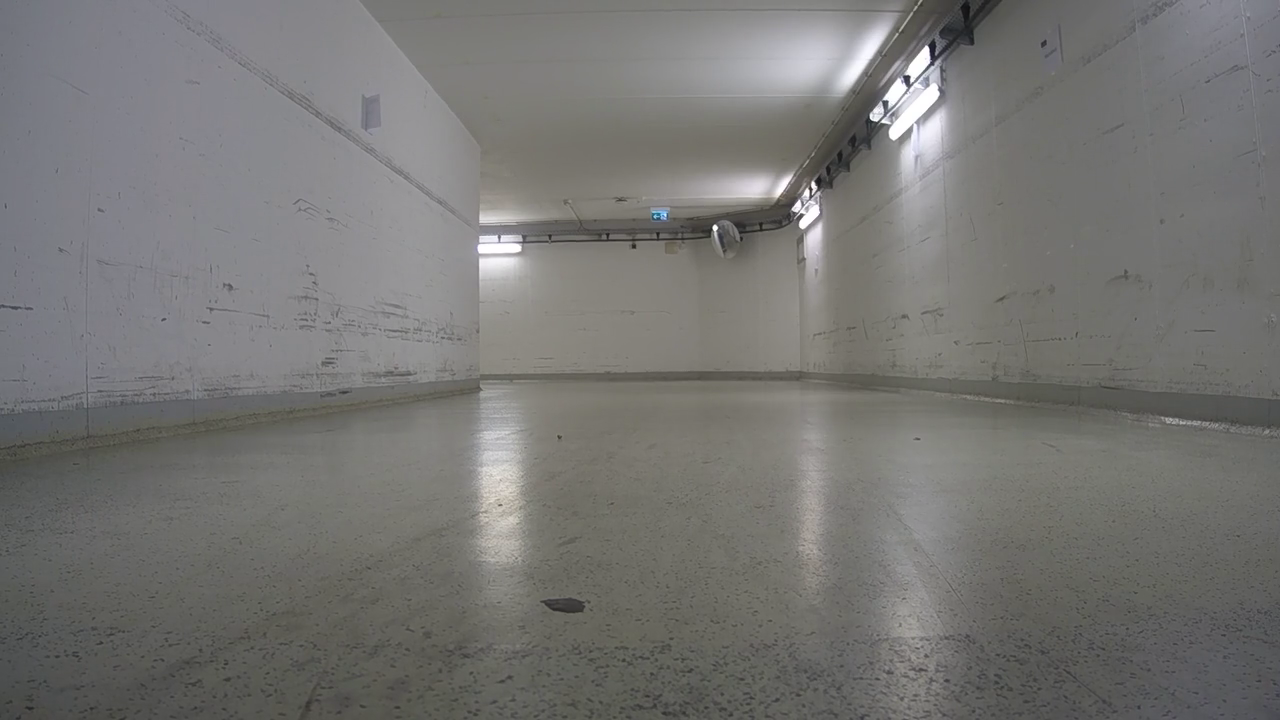
\includegraphics[width=\linewidth]{gang.png}
    \caption{Voorbeeld van een gang uit onze dataset.}
    \label{fig:gang}
\end{figure}

Deze detecties zullen we gebruiken om de locatie van de robot te tracken op basis van de informatie op de kaart op voorwaarde dat deze vertrekt op een gekende locatie.
Het tracken van de positie is het eindpunt voor dit onderzoek, maar deze informatie kan later gebruikt worden om de robot autonoom te navigeren naar een eindpunt.

\pagebreak
Hoe kan de positie van een mobiele robot te volgen in logistieke gangen van een ziekenhuis getrackt worden op basis van enkel een \gls{rgb} camera en een
semantische kaart?
Wat zijn de beste technieken om de waargenomen omgeving te koppelen aan informatie op de kaart?
Welke bijkomende informatie moet de kaart bevatten om een locatie te beschrijven?